\section{Overview}
In this section are present some screenshots by \textit{MOQA} mobile application.\\
During the design and development, the attention was focused on the mobile application, even if the application is developed to adapt itself to a larger screen. Layout, dimensions and colours are picked by the Apple Human Interface Guidelines.\\

\section{Mock-up}
At the beginning of the project, it was provided to the stakeholders a \textit{mock-up} (Figure \ref{img:initialWireframe}) of the application to have an approval that the draft was meeting the requirements and to show an overview of the flow of the application.

\begin{figure}[H]
\begin{center}
  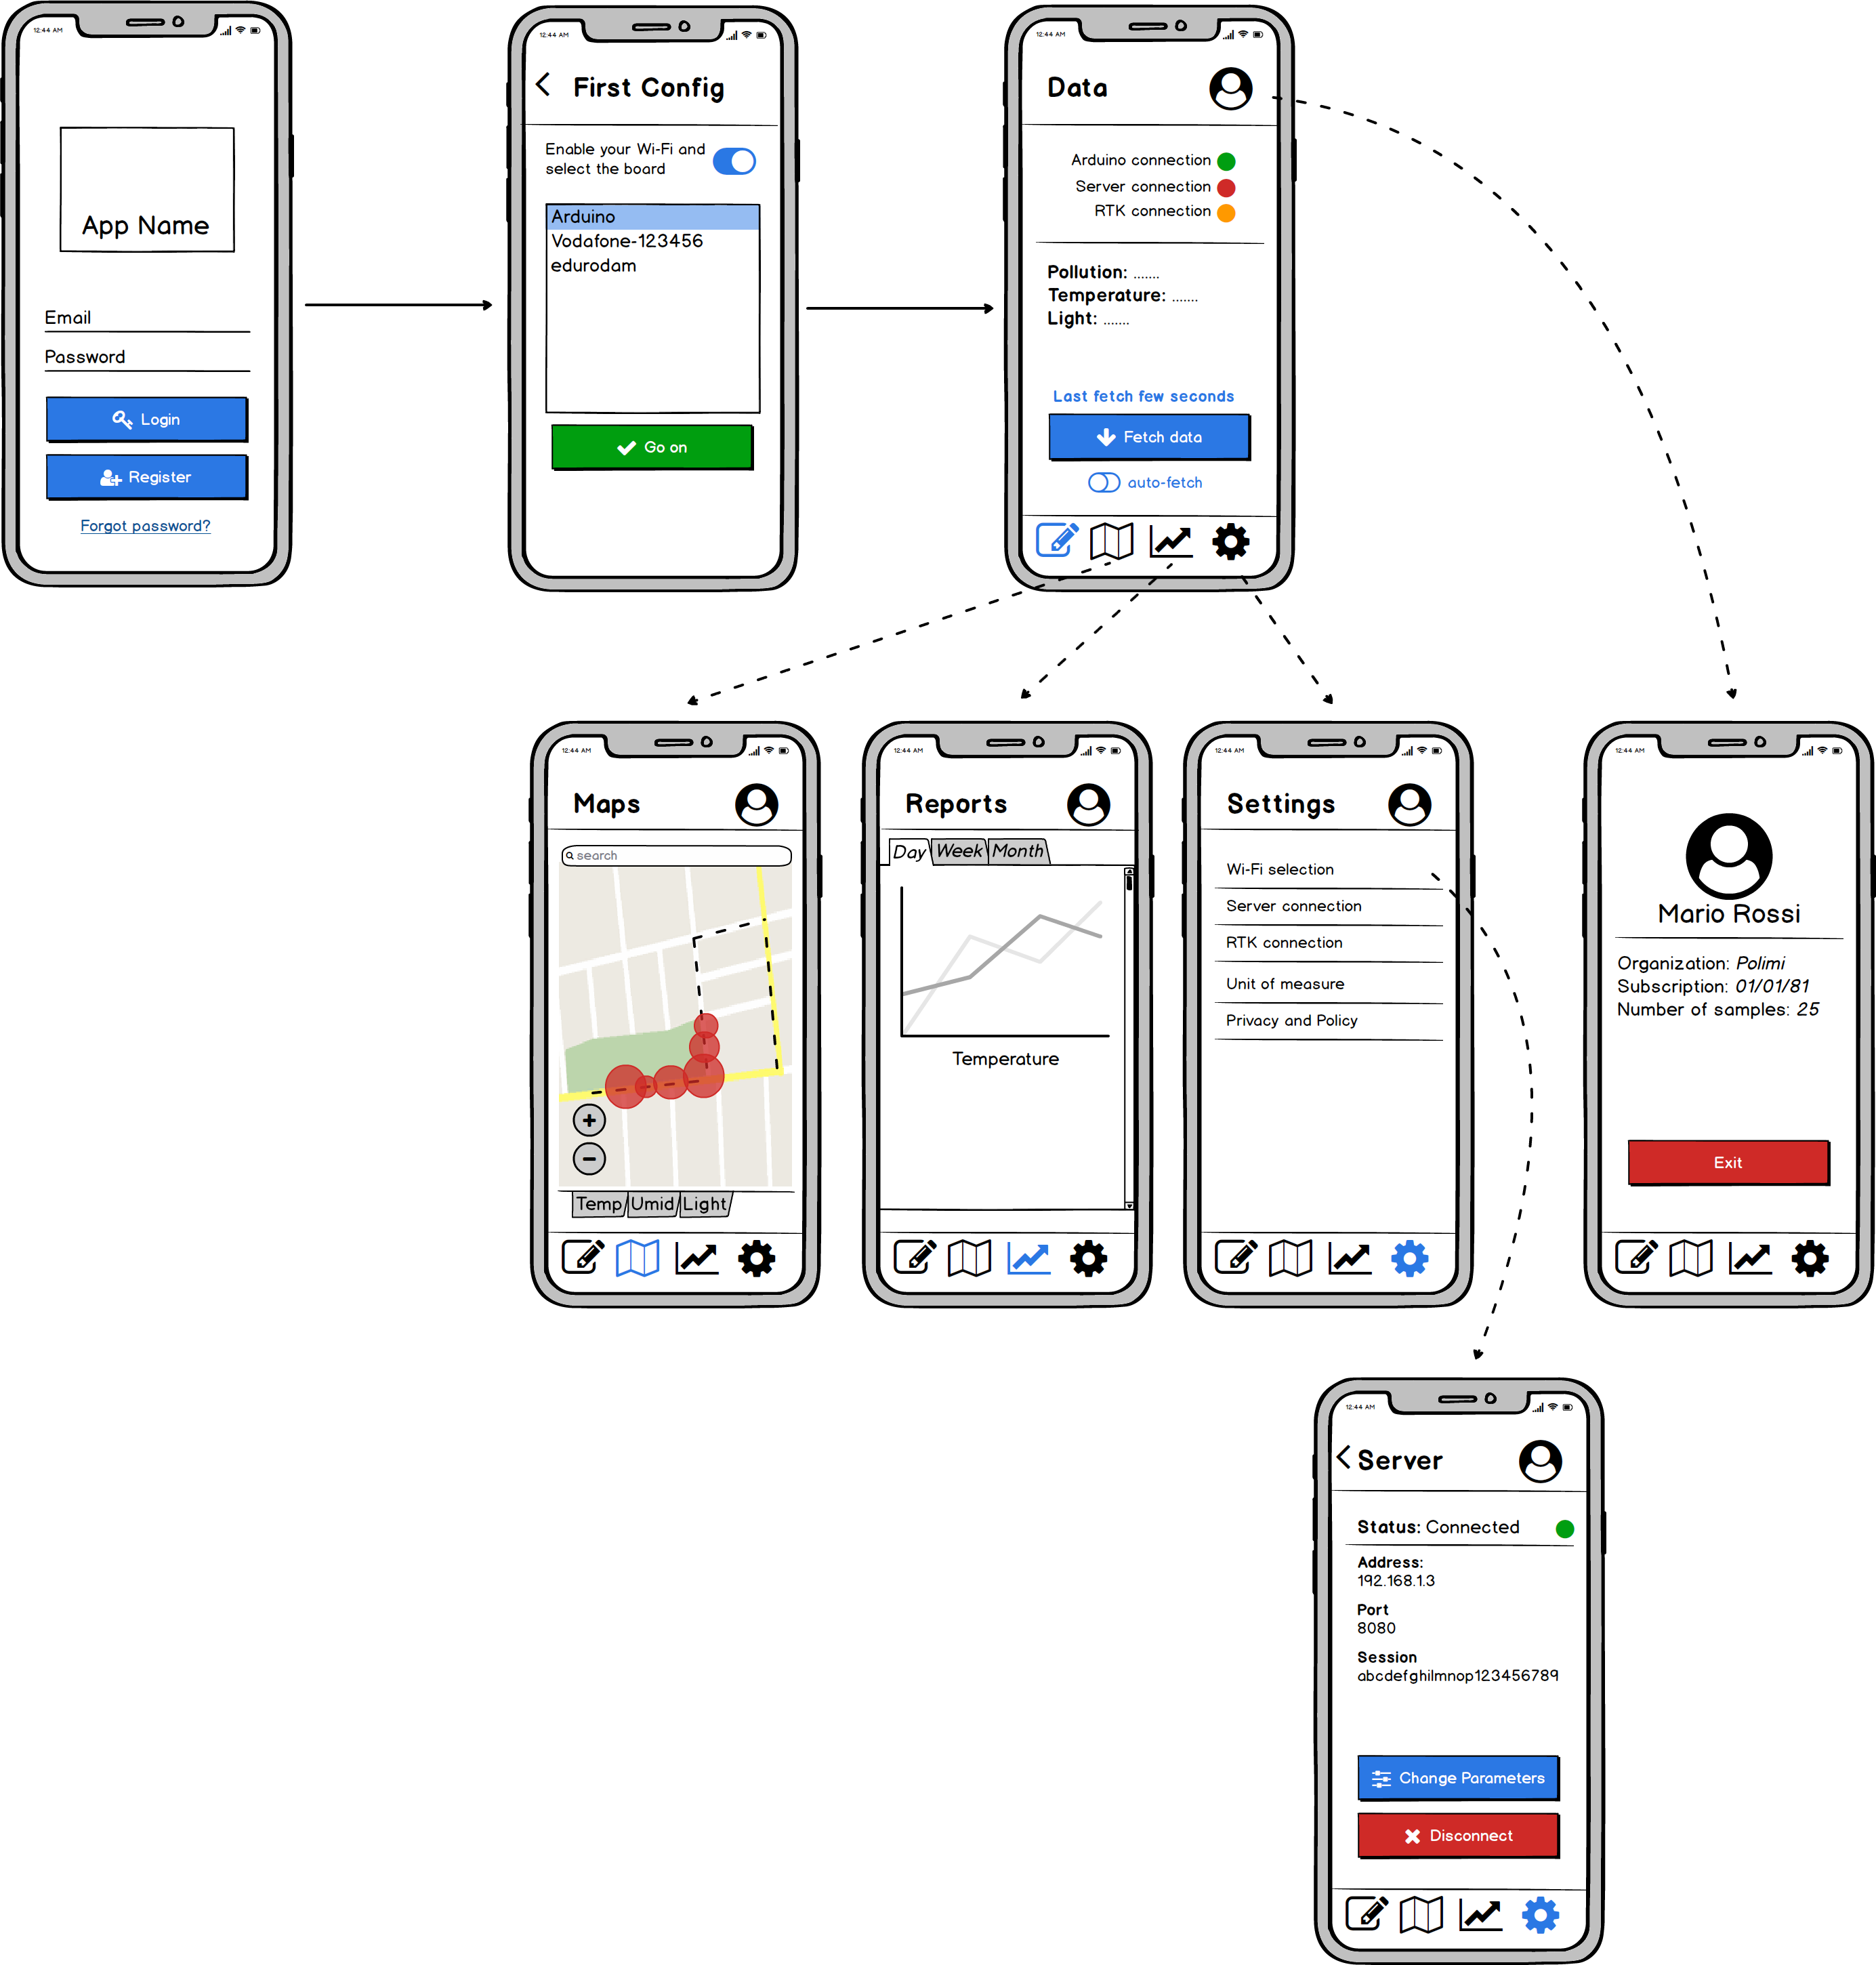
\includegraphics[width=\textwidth]{img/initialWireframe.png}
  \hspace{0.05\linewidth}
  \centering
  \caption{\textit{MOQA} initial mock-up}
  \label{img:initialWireframe}
\end{center}
\end{figure}
\clearpage

\section{Screens}

\begin{figure}[H]
\centering
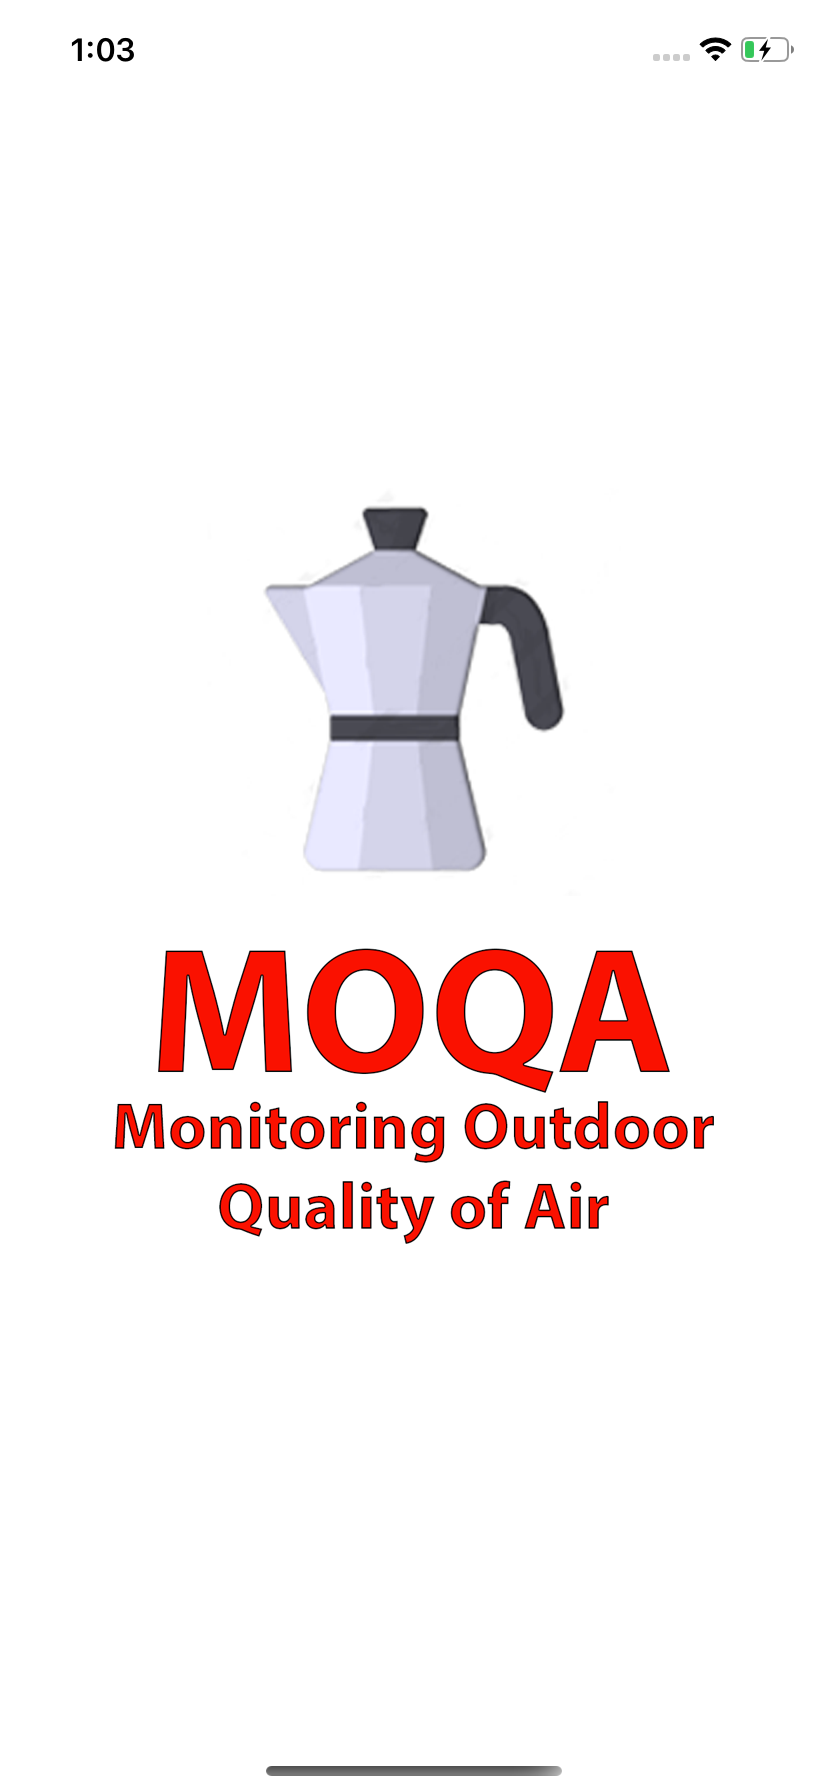
\includegraphics[height=.6\textheight]{./img/ui/splash.png}
\caption{\textbf{Splash Screen}}
\end{figure}
\begin{center}
The \textbf{Splash Screen} welcomes the user when the application is starting; meanwhile it restores the state of the application or loads the default one.    
\end{center}

\begin{figure}[H]
\centering
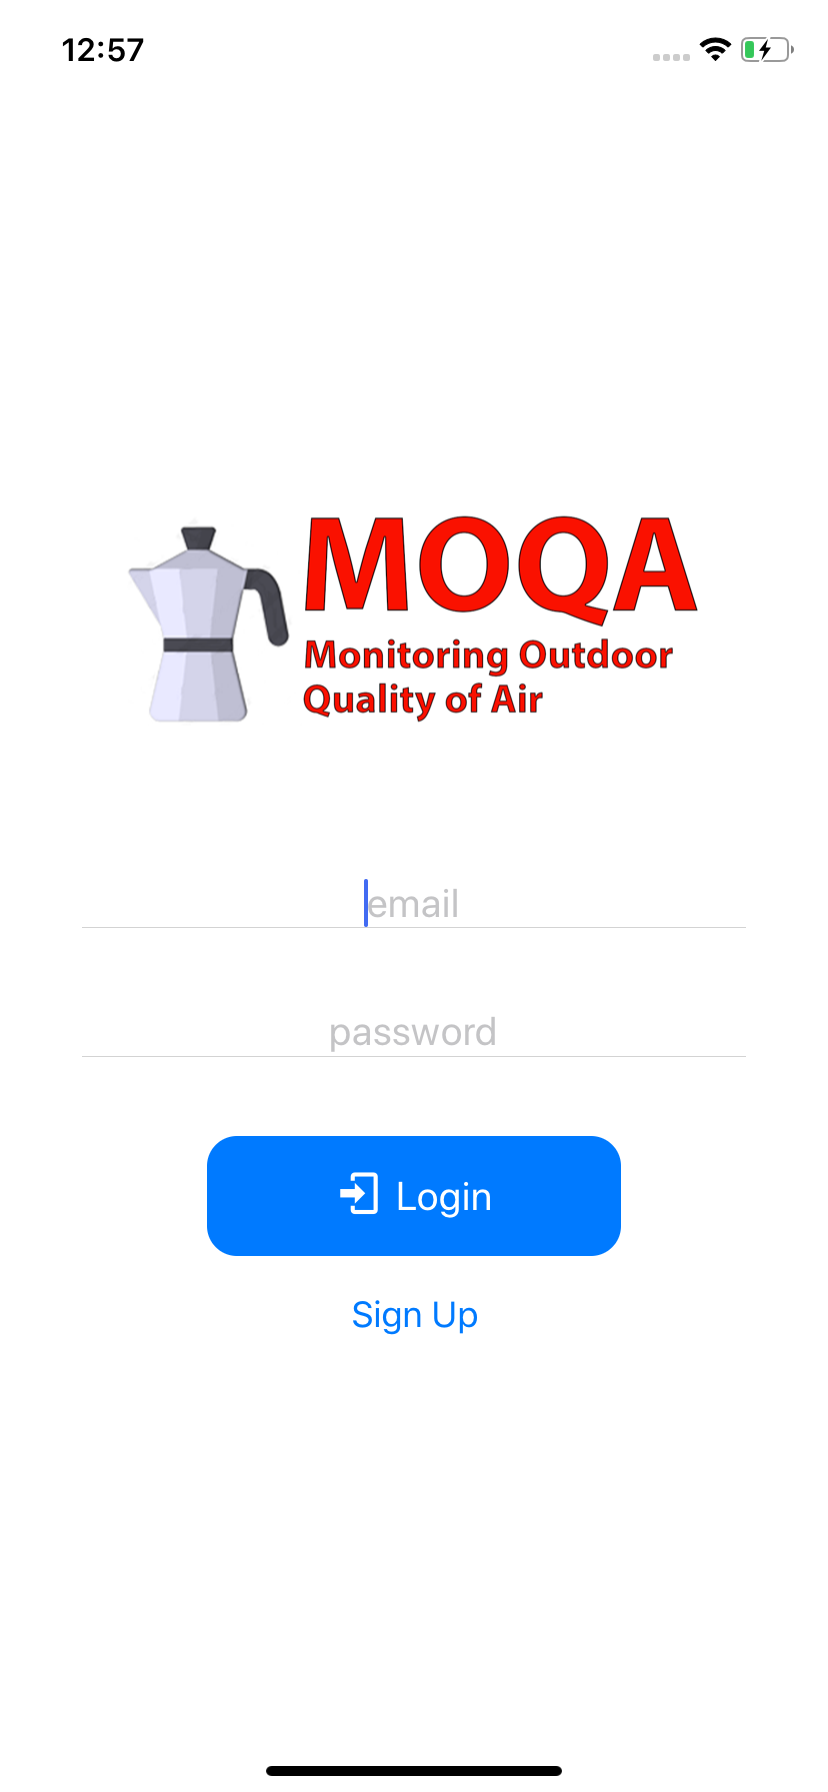
\includegraphics[height=.6\textheight]{./img/ui/login.png}
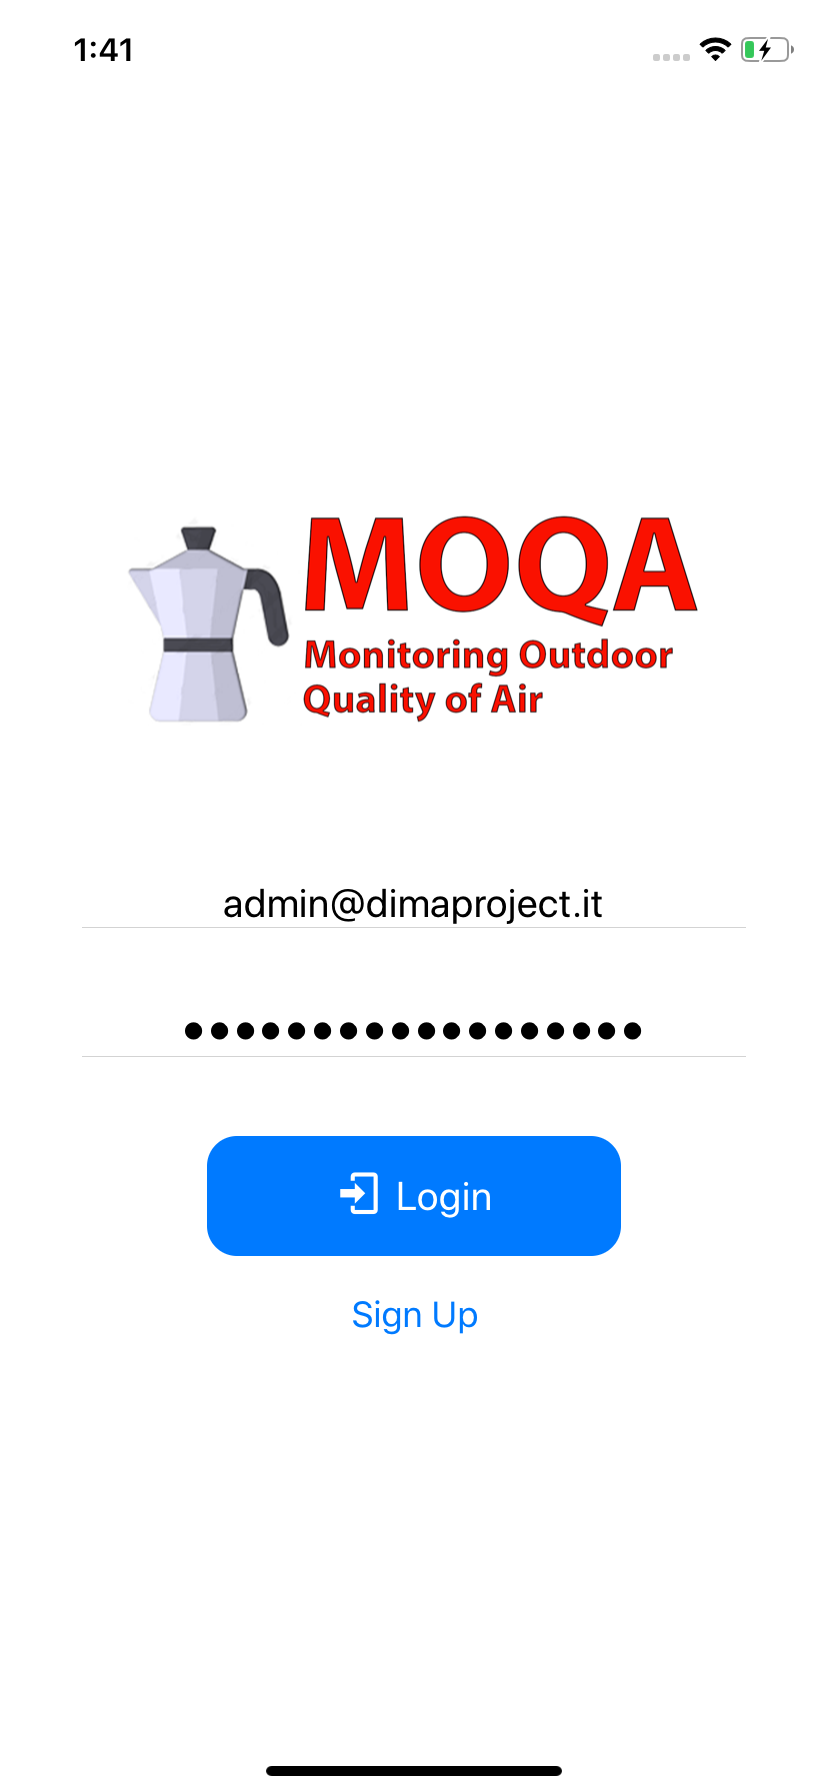
\includegraphics[height=.6\textheight]{./img/ui/login2.png}
\caption{\textbf{Login Screen}}
\end{figure}
\begin{center}
The \textbf{Login Screen} is the first screen that the user sees after the application is loaded. The user could enter its credential or, if they are in memory, the application fills the fields.
\end{center}

\begin{figure}[H]
\centering
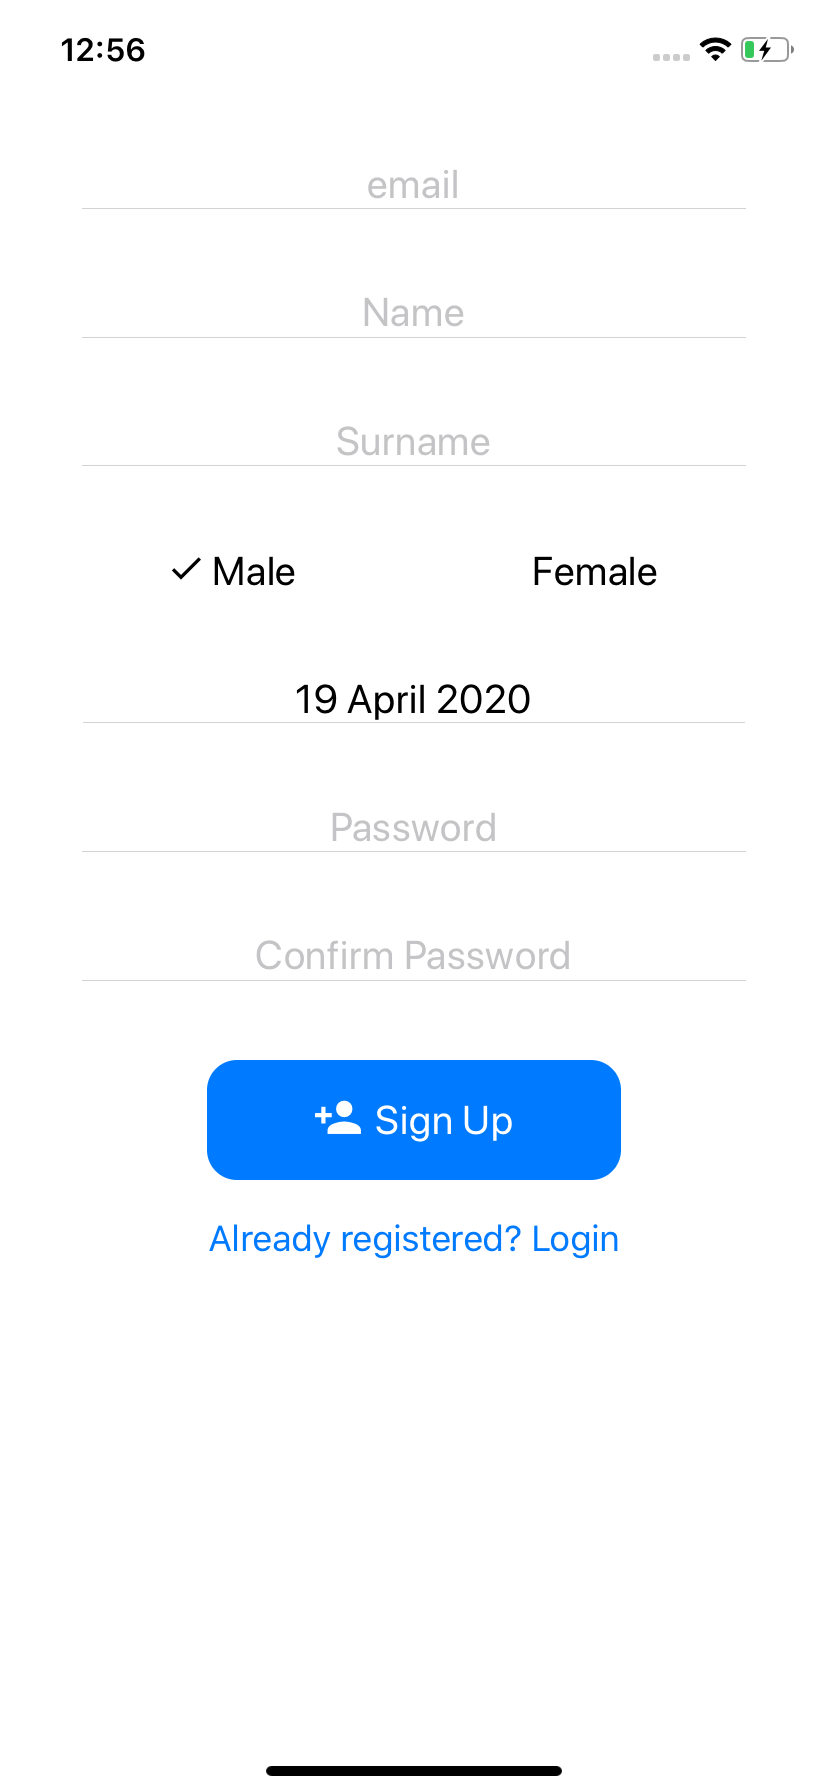
\includegraphics[height=.6\textheight]{./img/ui/signup.png}
\caption{\textbf{Sign Up Screen}}
\end{figure}
\begin{center}
The \textbf{Sign Up Screen} allows the user to register in the application.
\end{center}

\begin{figure}[H]
\centering
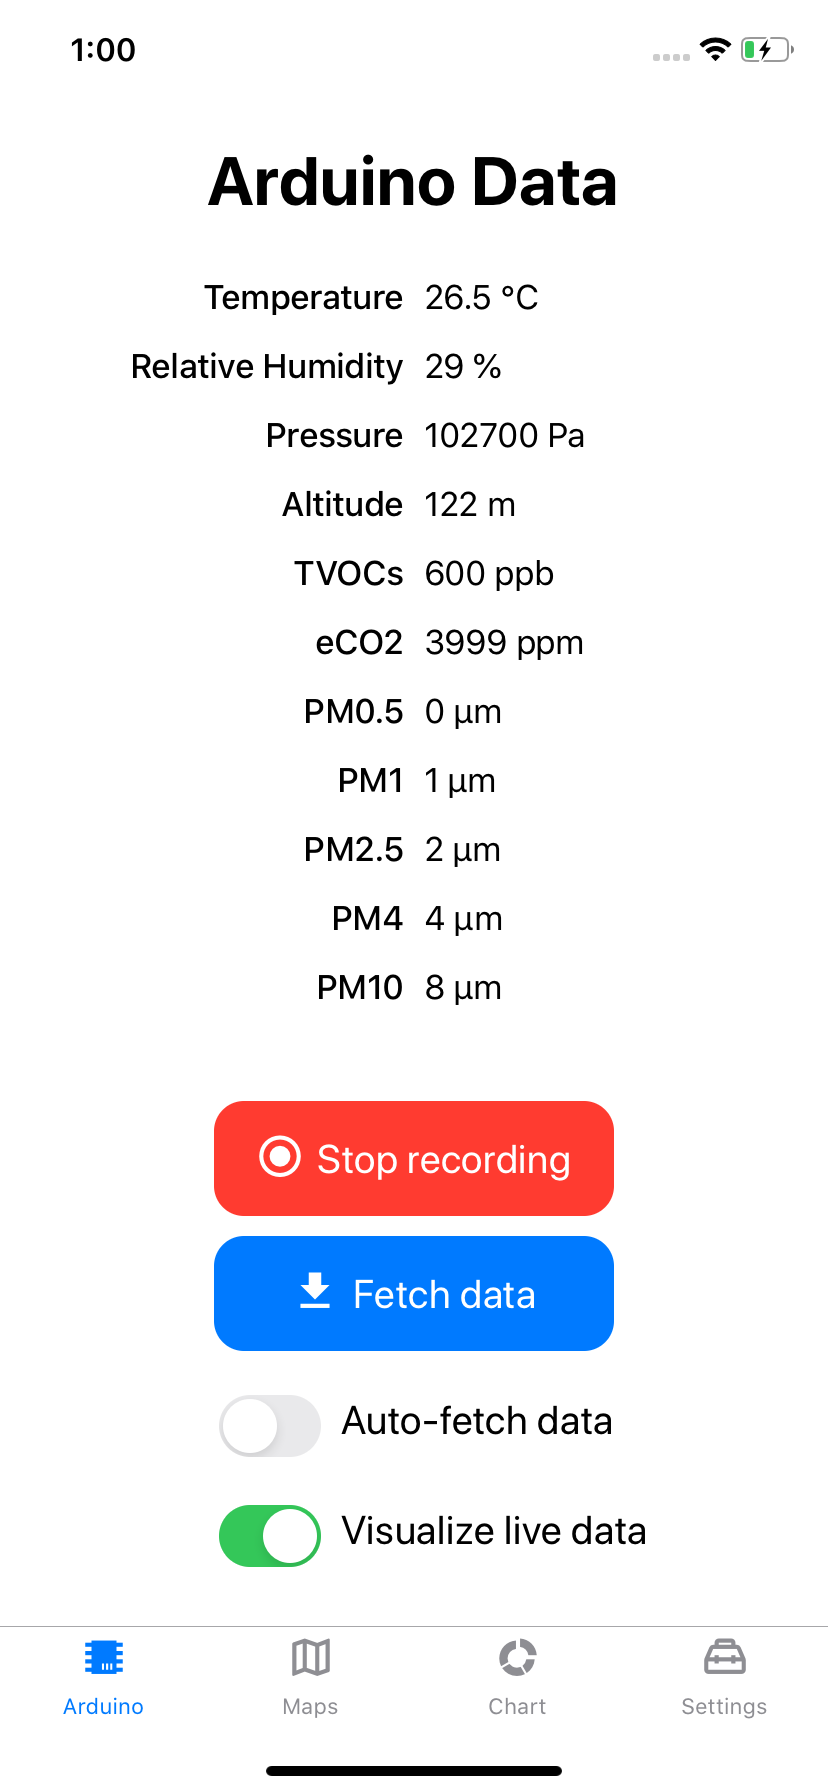
\includegraphics[height=.6\textheight]{./img/ui/arduino_data.png}
\caption{\textbf{Arduino Screen}}
\end{figure}
\begin{center}
The \textbf{Arduino Screen} displays the data coming from the \textit{Arduino} board, if available.\\
It allows the user to start/stop the recording of data (it means that the data gathered by the board are sent to the server).\\
It allows the user to \textit{Fetch data} (it is a manual request of data to the board) or enable the \textit{Auto-fetch data} that starts a routine that every second refreshes the data from the board.\\
Moreover in this screen, the user could decide if it wants to visualize the live data from the board or the data stored in the server in the \textbf{Map Screen} and \textbf{Chart Screen}.
\end{center}

\begin{figure}[H]
\centering
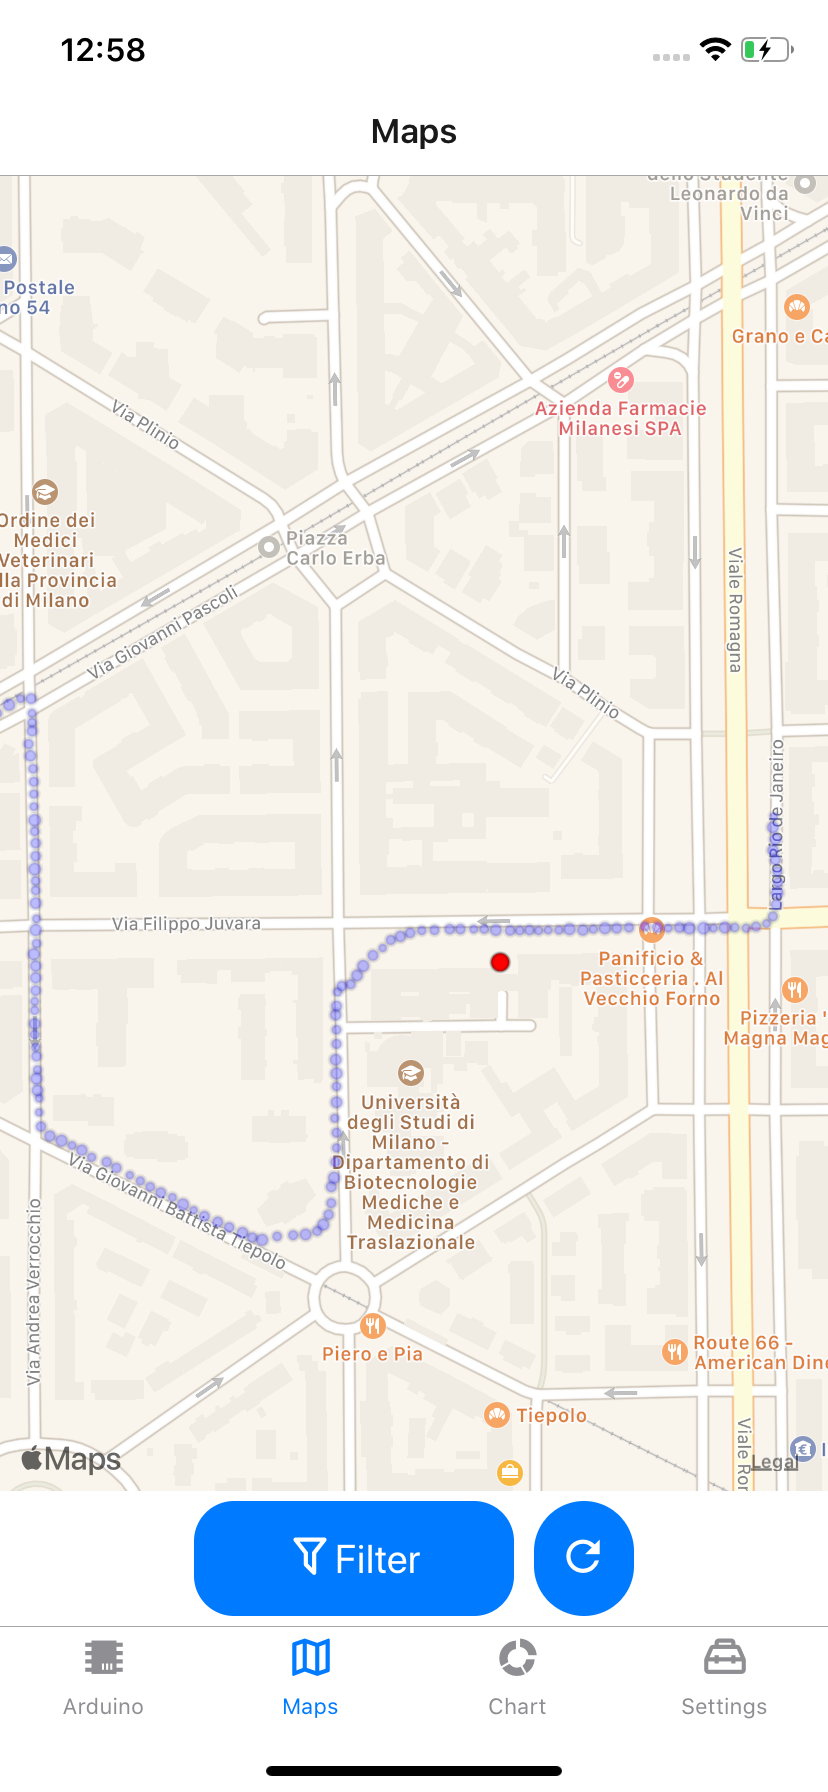
\includegraphics[height=.6\textheight]{./img/ui/map.png}
\caption{\textbf{Map Screen}}
\end{figure}
\begin{center}
The \textbf{Map Screen} displays the data coming from the \textit{Arduino} board (blue circles) and \textit{ARPA} dataset (red circles) on a map. The radius of a circle depends on the value of the data it is associated.\\
The user could filter the data clicking on the \textit{Filter} button and could refresh the map with the blue button on the right.
\end{center}

\begin{figure}[H]
\centering
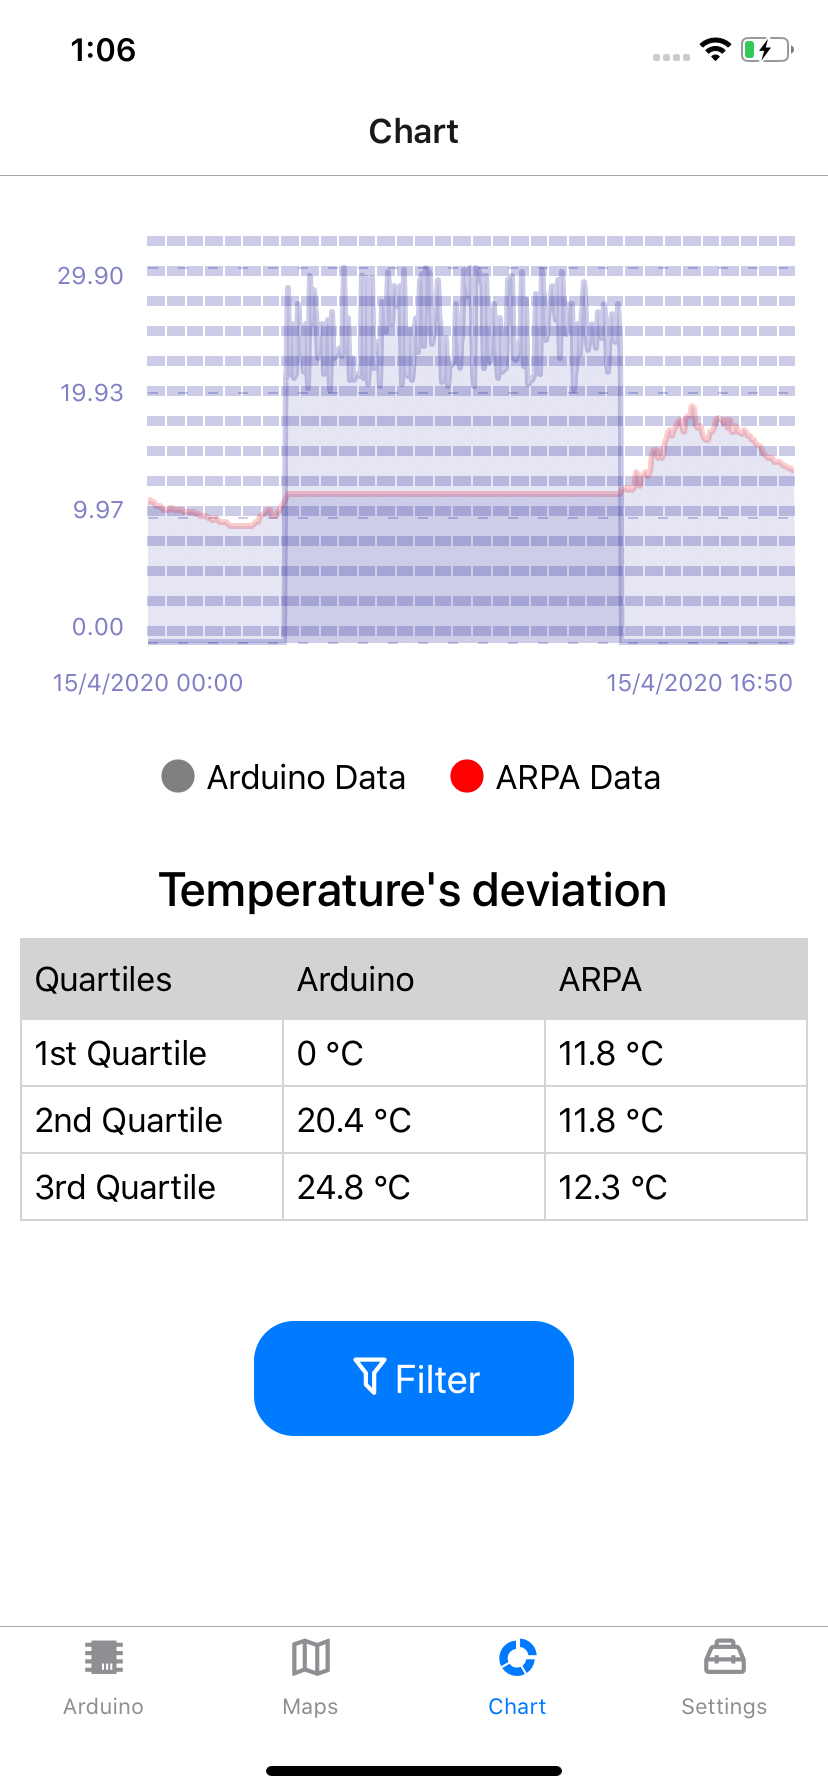
\includegraphics[height=.6\textheight]{./img/ui/chart.png}
\caption{\textbf{Chart Screen}}
\end{figure}
\begin{center}
The \textbf{Chart Screen} displays the data coming from the \textit{Arduino} board and \textit{ARPA} dataset on a graph. Moreover, it provides a table with a computation of the quartile deviation.\\
The user could filter the data clicking on the \textit{Filter} button and could refresh the page scrolling-up.
\end{center}

\begin{figure}[H]
\centering
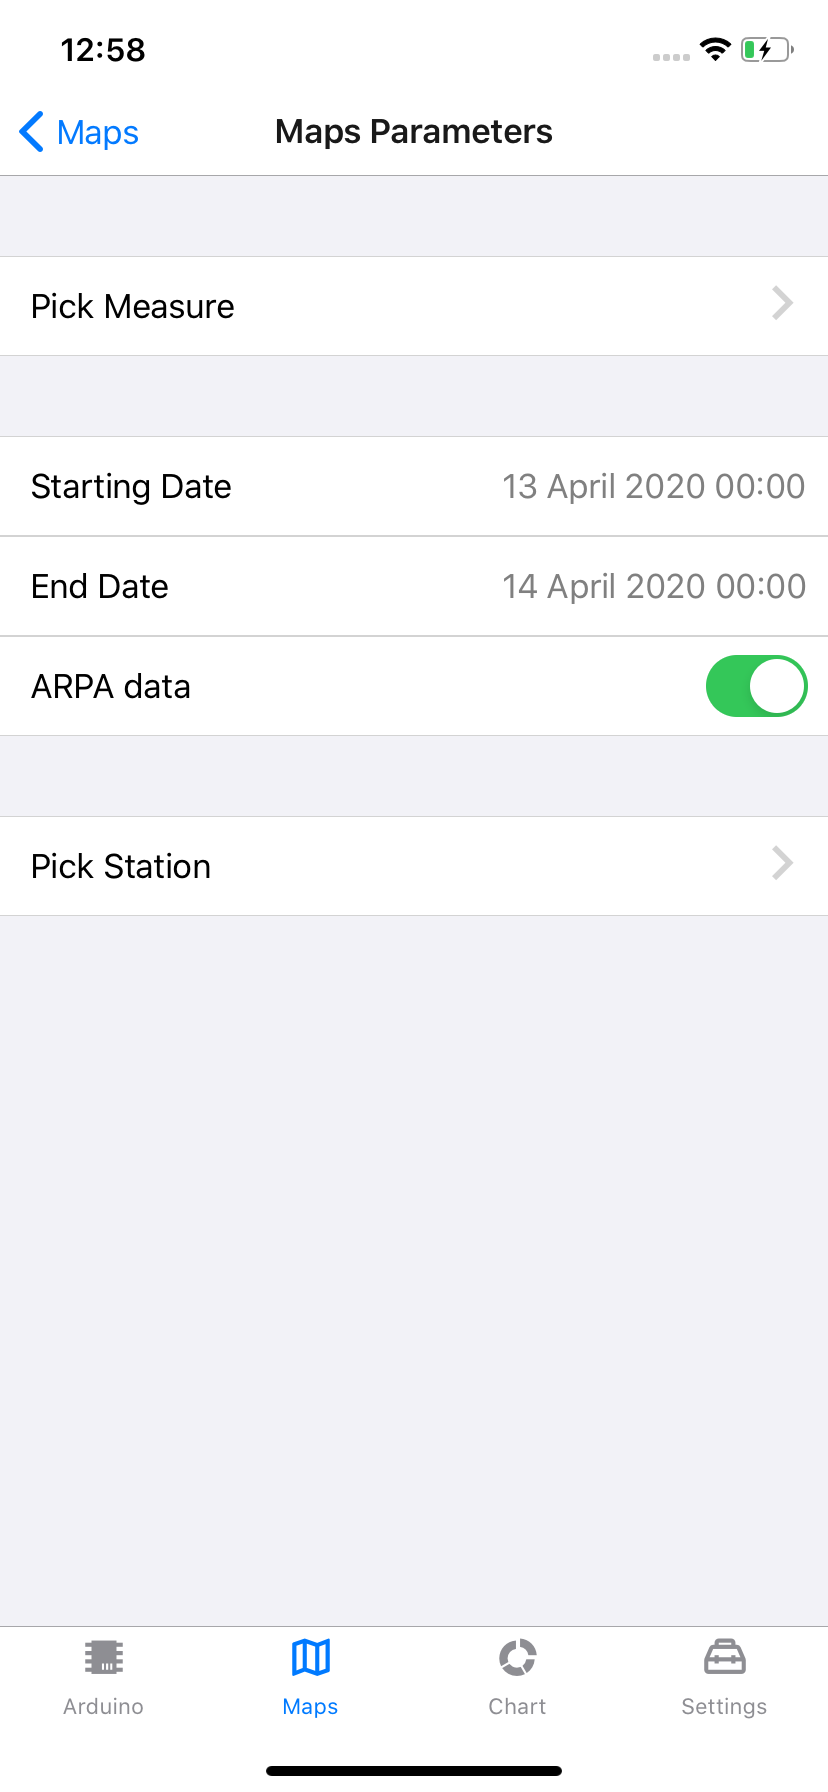
\includegraphics[height=.6\textheight]{./img/ui/filter.png}
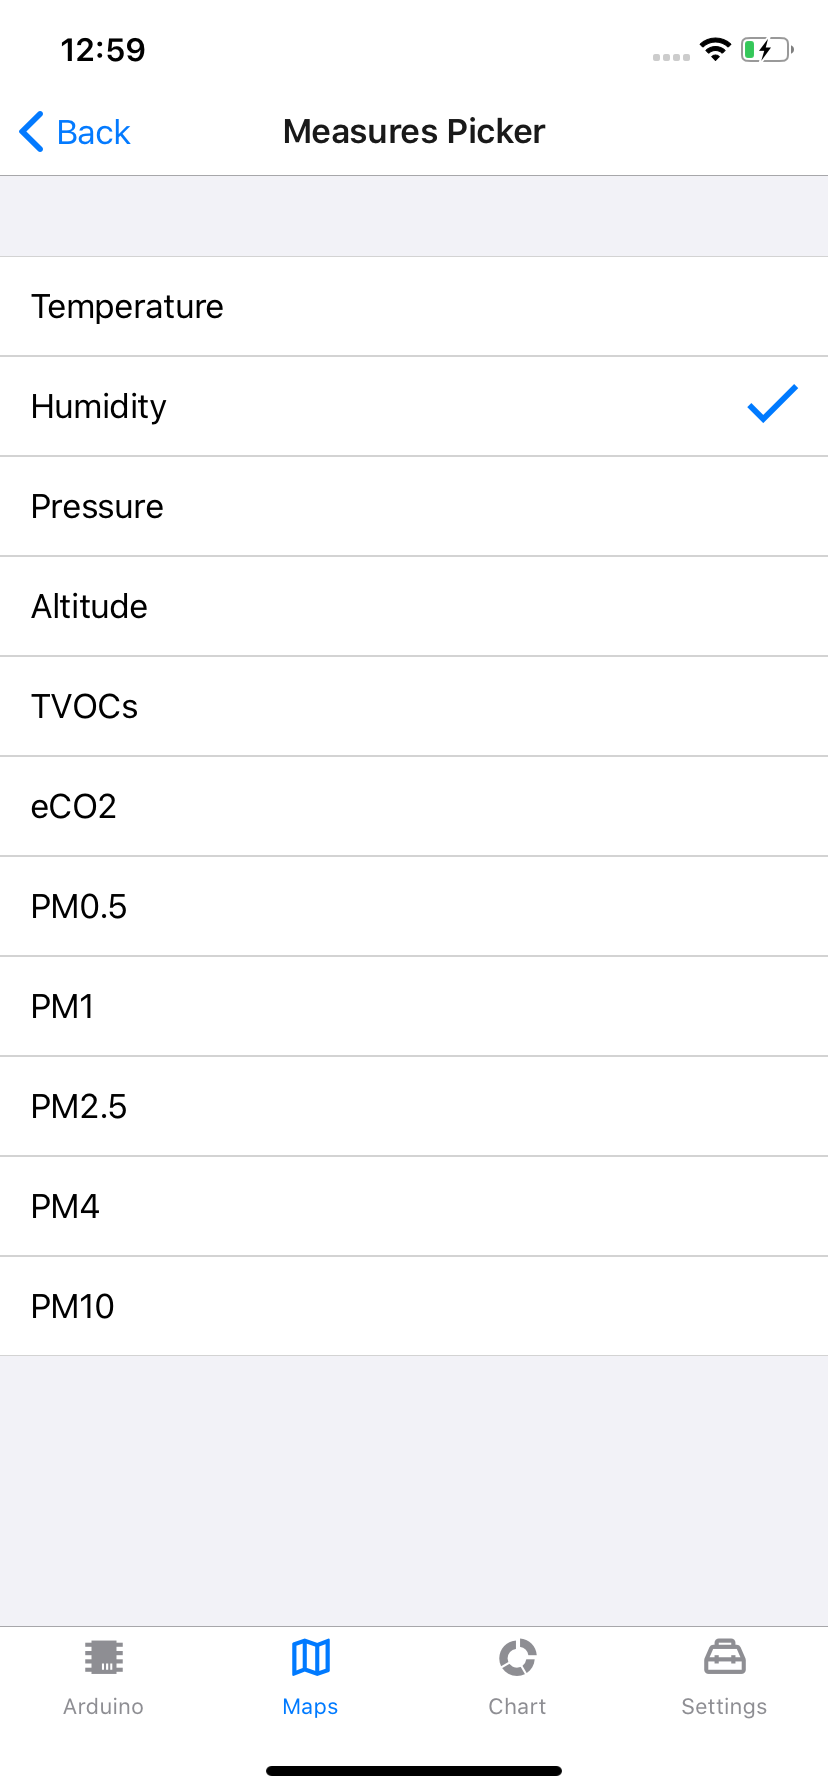
\includegraphics[height=.6\textheight]{./img/ui/mea_picker.png}
\caption{\textbf{Filter Screens}}
\end{figure}
\begin{center}
The \textbf{Filter Screens} allow the user to set the parameters to limit the data visualized in the \textbf{Map Screen} and \textbf{Chart Screen}.\\
The user could pick the measure it wants to visualize, select the time range and decide to visualize the ARPA data defining the station.\\
In the application the \textbf{Filter Screen} is used by the \textbf{Map Screen} and the \textbf{Chart Screen}
\end{center}

\begin{figure}[H]
\centering
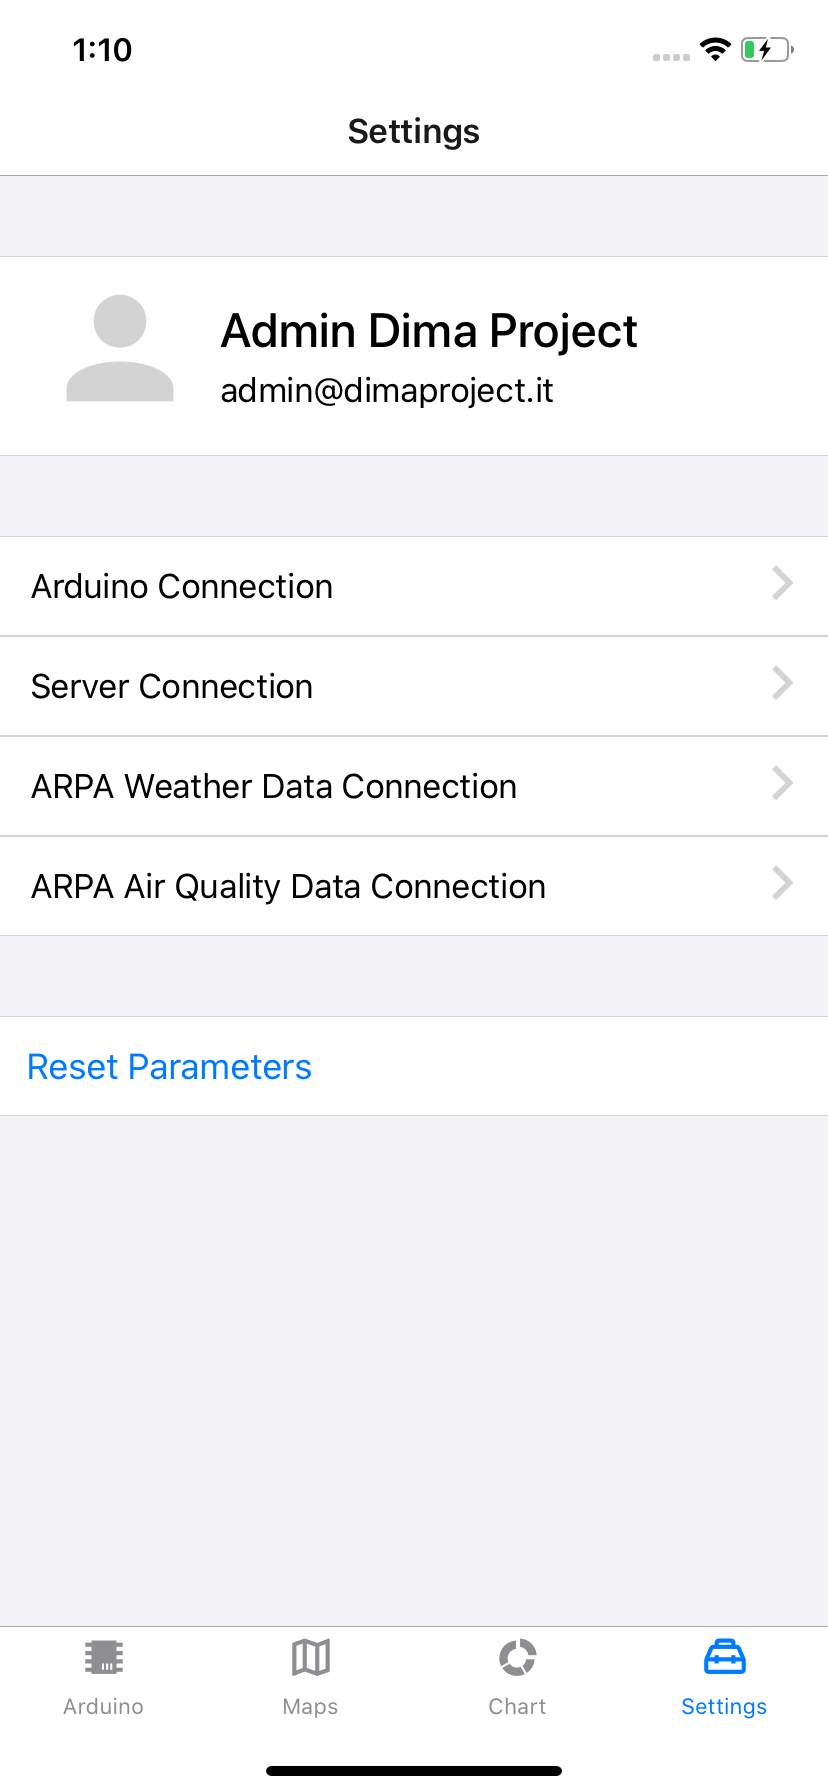
\includegraphics[height=.6\textheight]{./img/ui/settings.png}
\caption{\textbf{Settings Screen}}
\end{figure}
\begin{center}
The \textbf{Settings Screen} allows the user to visualize and to change different parameters of the application.\\
The user could also decide to reset the parameters to an initial and default state.
\end{center}

\begin{figure}[H]
\centering
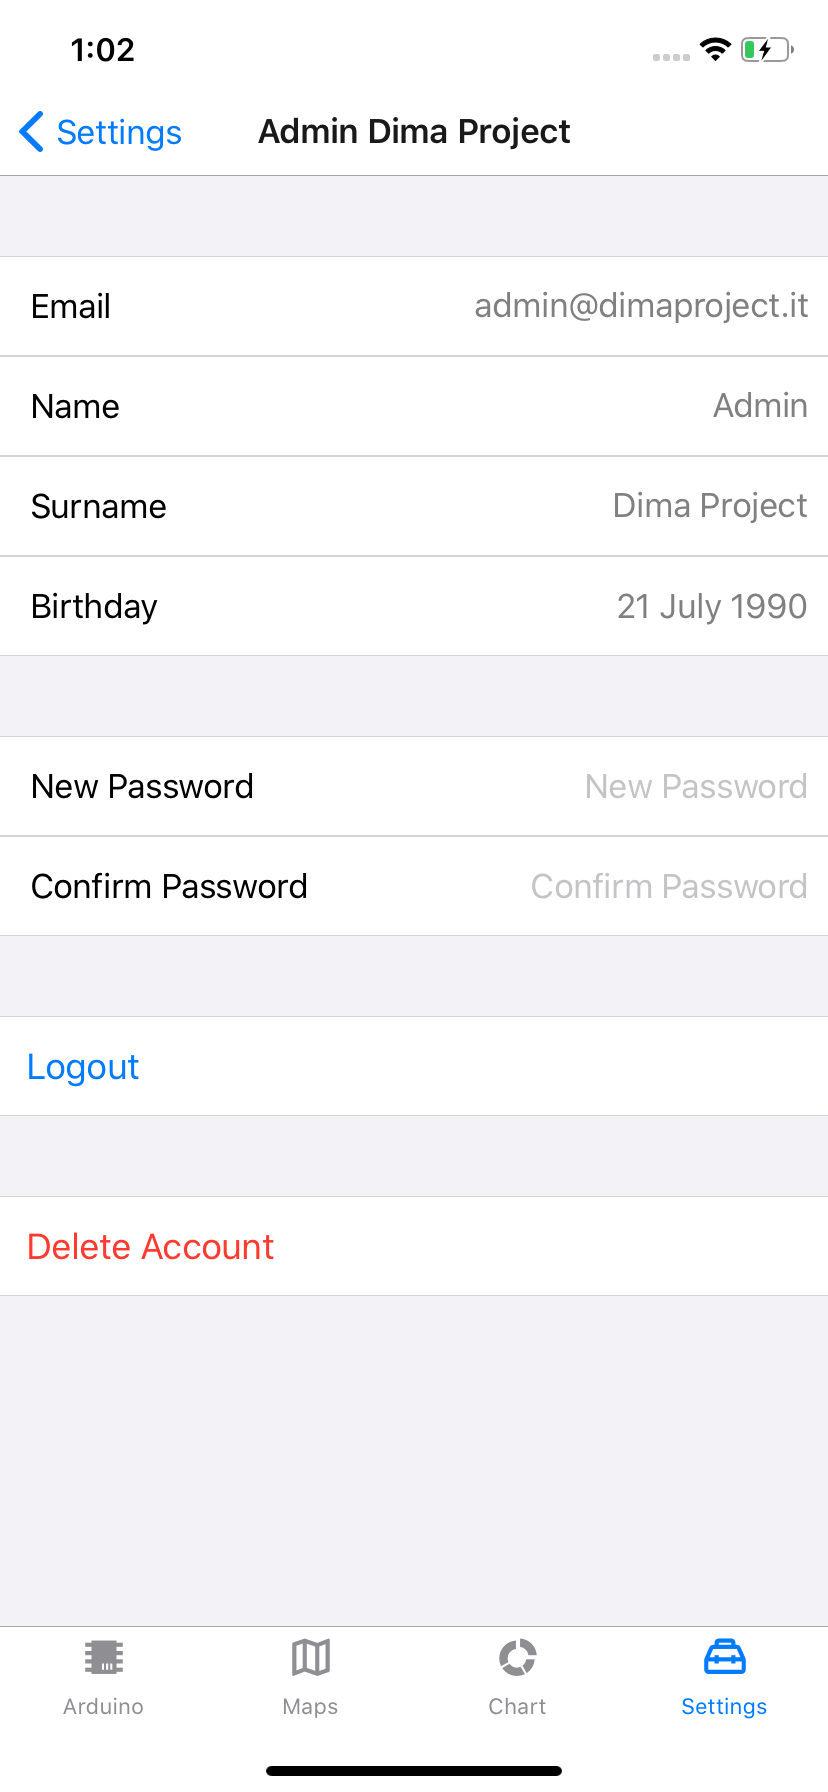
\includegraphics[height=.6\textheight]{./img/ui/user_settings.png}
\caption{\textbf{User Settings Screen}}
\end{figure}
\begin{center}
The \textbf{User Settings Screen} allows the user to visualize and to change the information about its account. Moreover it allows the user to delete its account or logout from the application.
\end{center}

\begin{figure}[H]
\centering
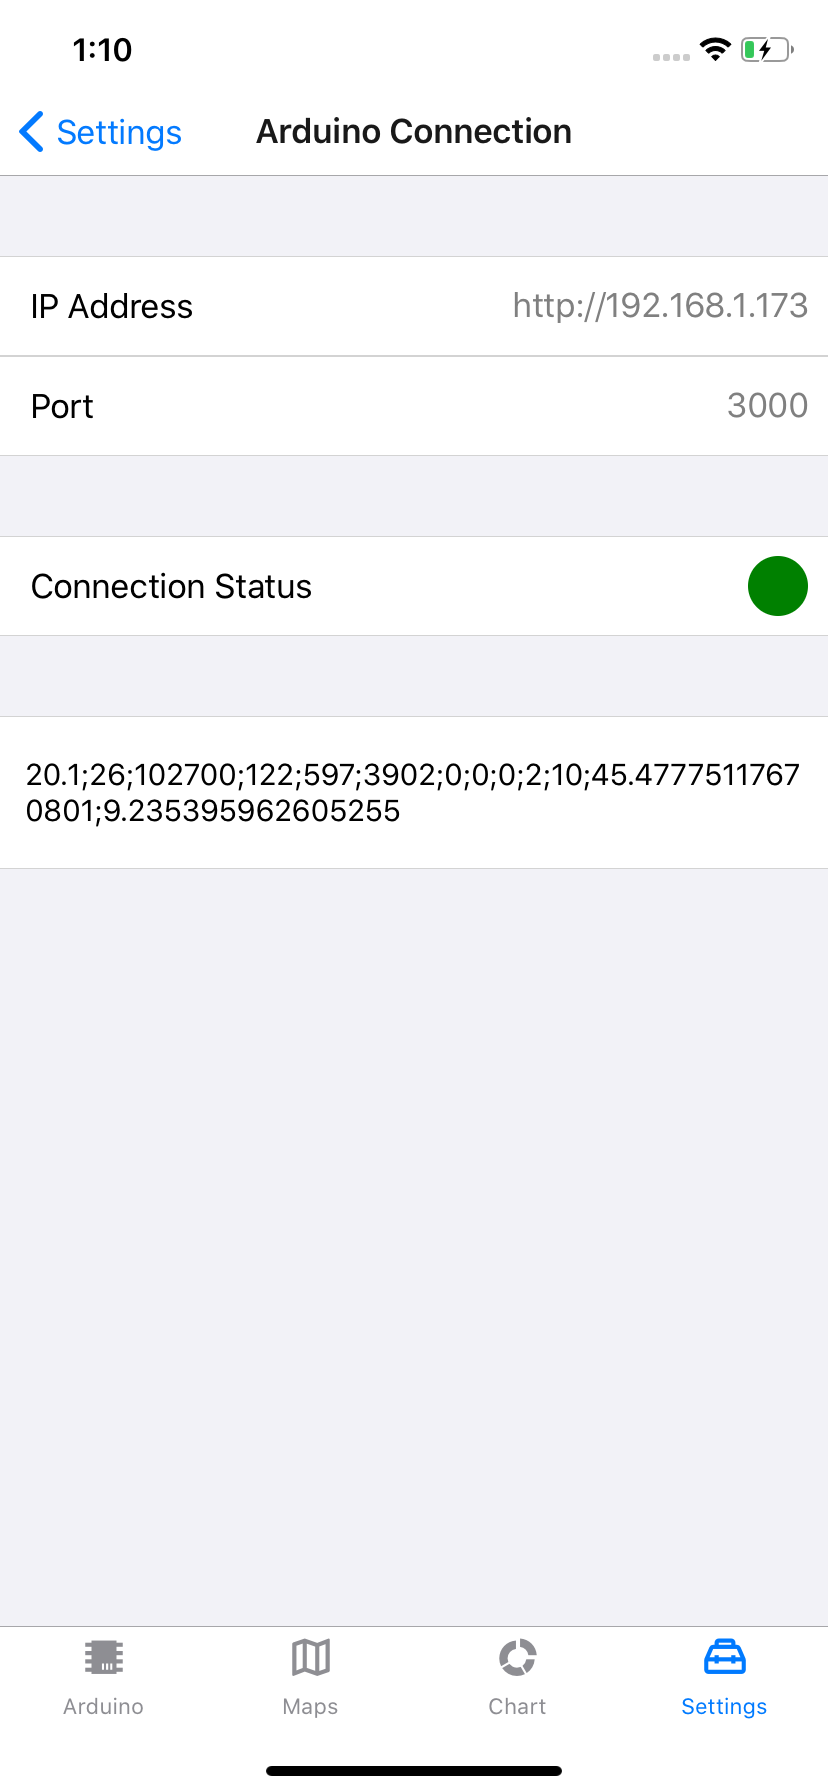
\includegraphics[height=.6\textheight]{./img/ui/arduino_settings.png}
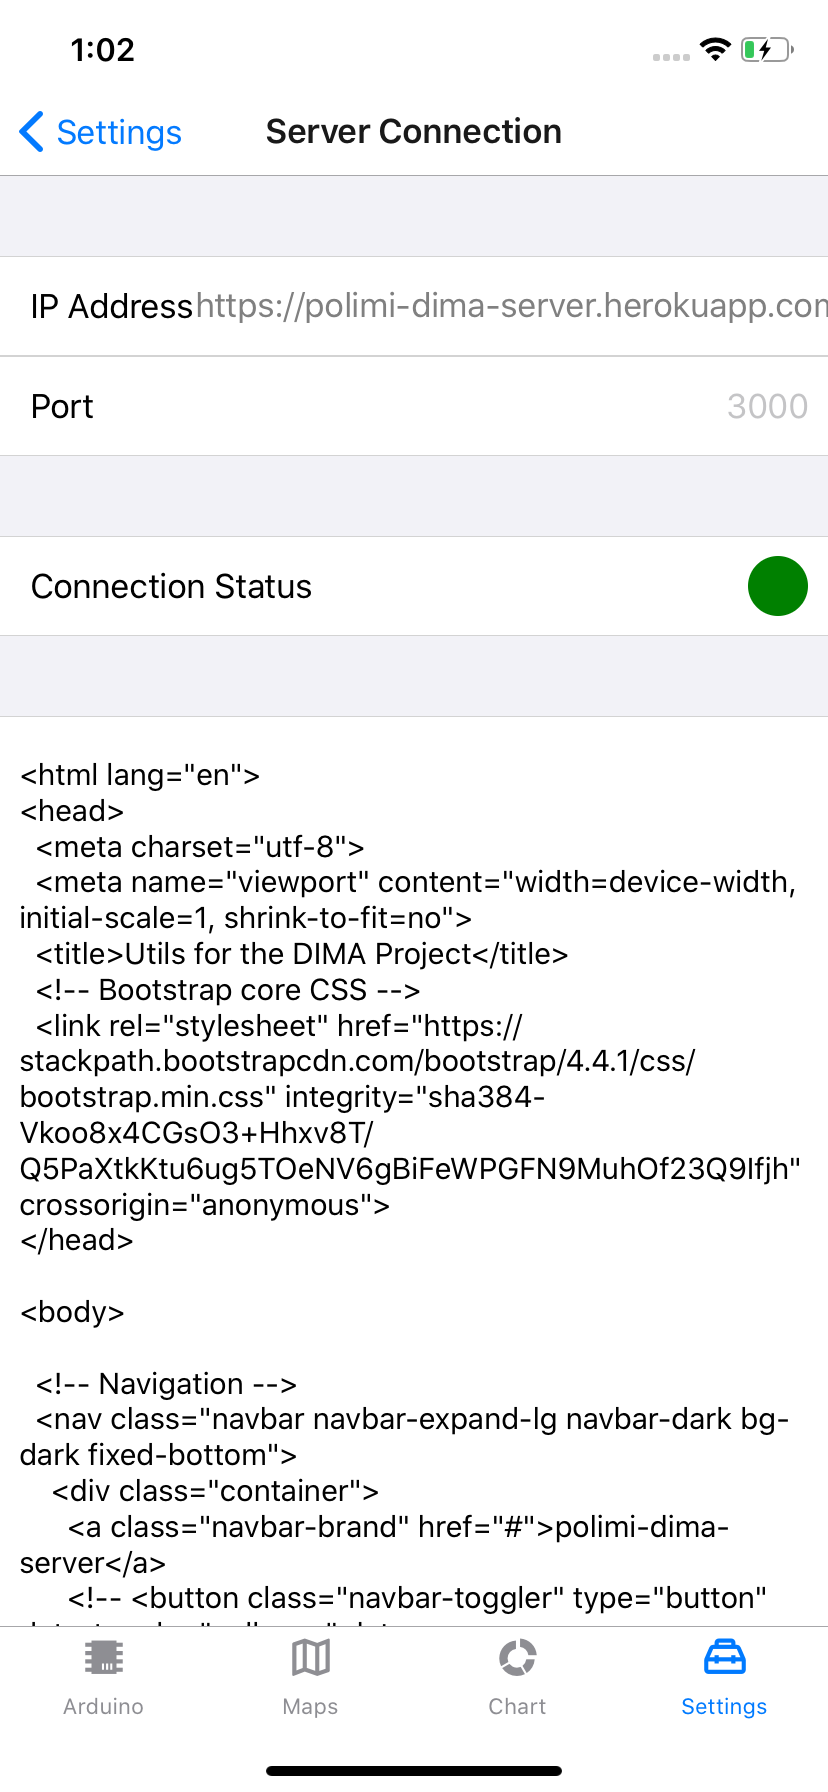
\includegraphics[height=.6\textheight]{./img/ui/server.png}
\caption{\textbf{Connection Screens}}
\end{figure}
\begin{center}
The \textbf{Arduino Connection Screen} and \textbf{Server Connection Screen} allow the user to change the IP address and the port of the \textit{Arduino} board and the \textit{Application Server}.
\end{center}

\begin{figure}[H]
\centering
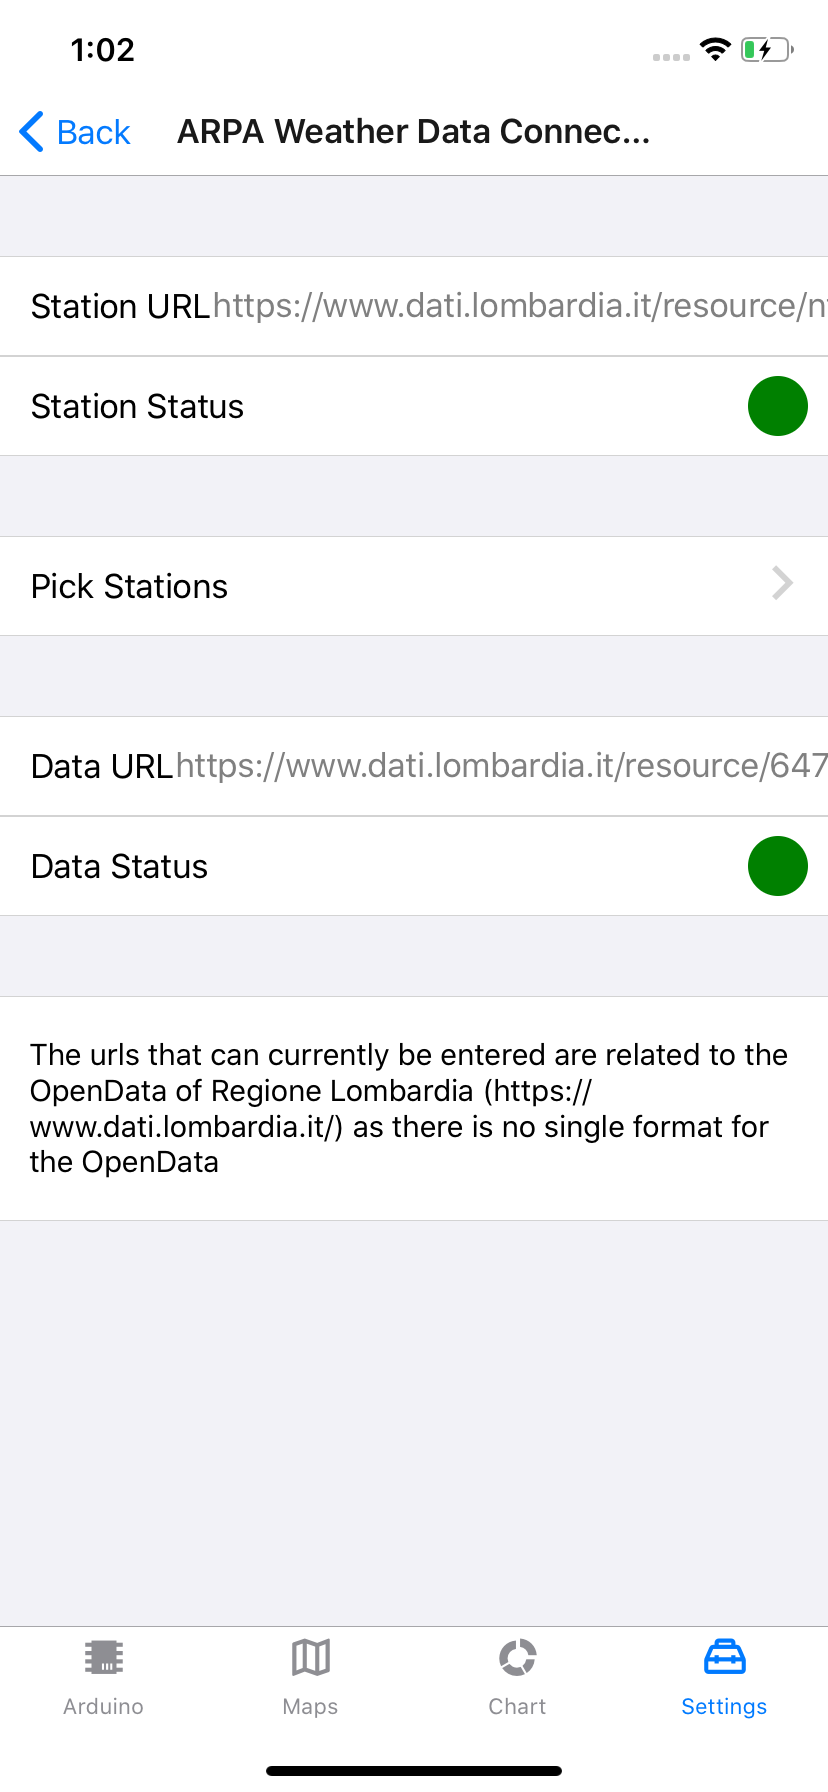
\includegraphics[height=.6\textheight]{./img/ui/arpa_settings.png}
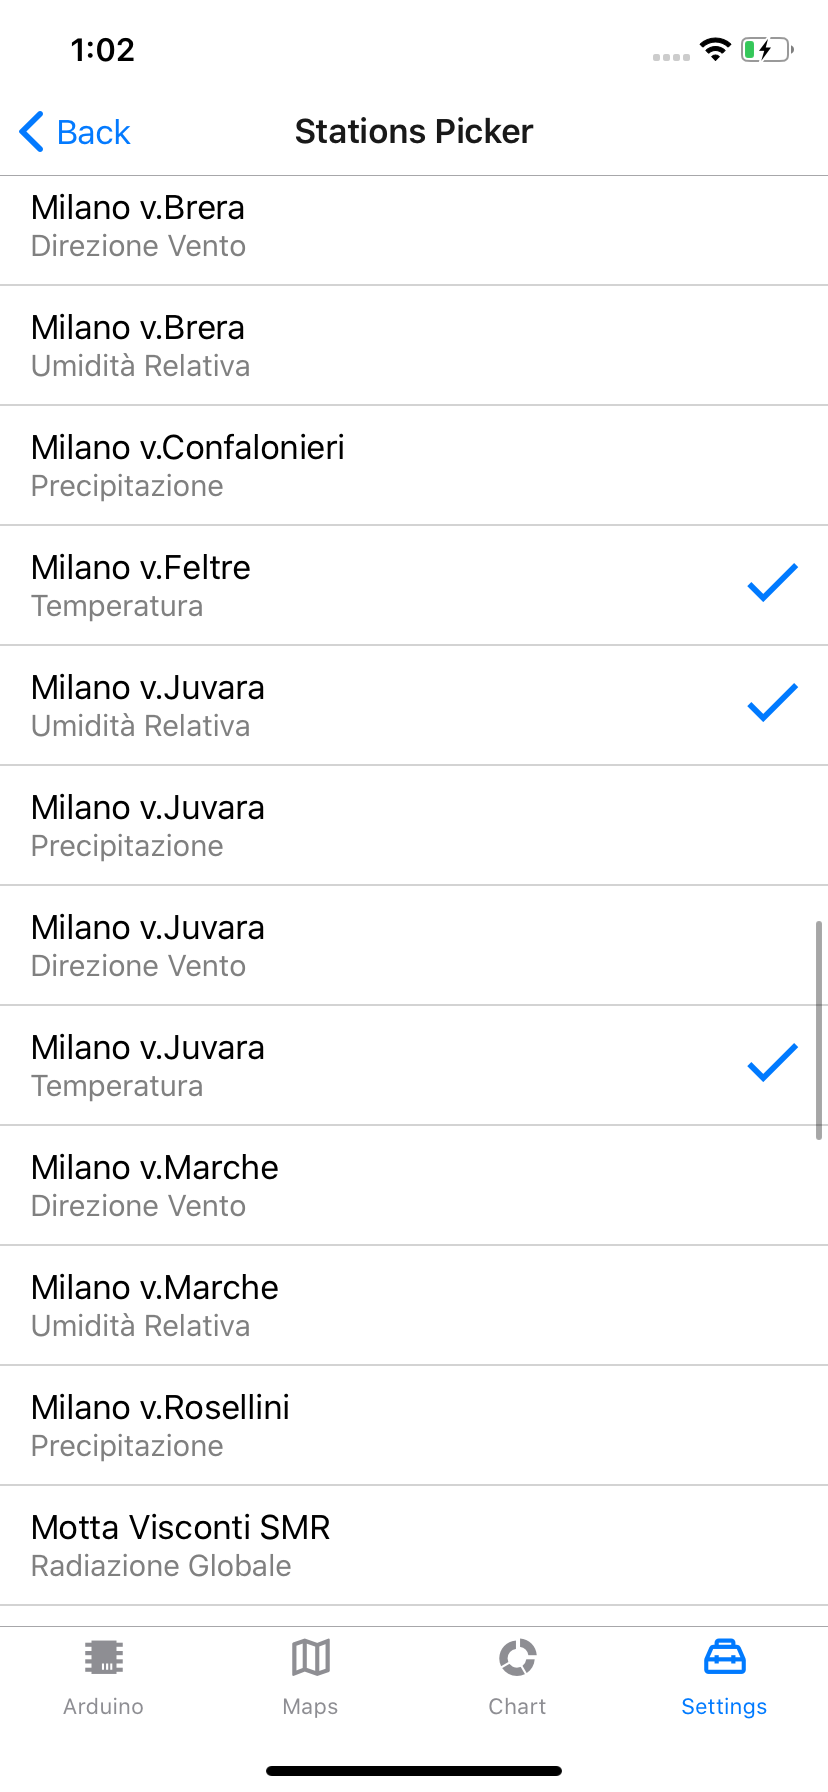
\includegraphics[height=.6\textheight]{./img/ui/stations_picker.png}
\caption{\textbf{ARPA Data Connection Screen}}
\end{figure}
\begin{center}
The \textbf{ARPA Data Connection Screen} allows the user to visualize and change the links of the stations and the data from \textit{Regione Lombardia} OpenData portal.\\ Moreover with the \textbf{Stations Picker Screen} allows the user to select the stations it wants to visualize in the \textbf{Pick Station Screen} of \textbf{Filter Screen}.\\
In the application there are two different \textit{screens}: one for the weather links and an other for the air quality links; however they are managed by the same \textit{Vue Native} component.
\end{center}